\begin{frame}[c]
	\myframetitle{Firefox Plugin for language detection}{German}
	%\usepackage{graphics} is needed for \includegraphics
\begin{figure}[htp]
\begin{center}
  
\includegraphics[scale=0.4]{../task05/ke_homepage.png} 
  \caption{The plugin detects german as language for the WebMining Website}
  \label{f:keHomepage}
\end{center}
\end{figure}
	
	
\end{frame}

\begin{frame}[c]
	\myframetitle{Firefox Plugin for language detection}{English}
	%\usepackage{graphics} is needed for \includegraphics
\begin{figure}[htp]
\begin{center}
  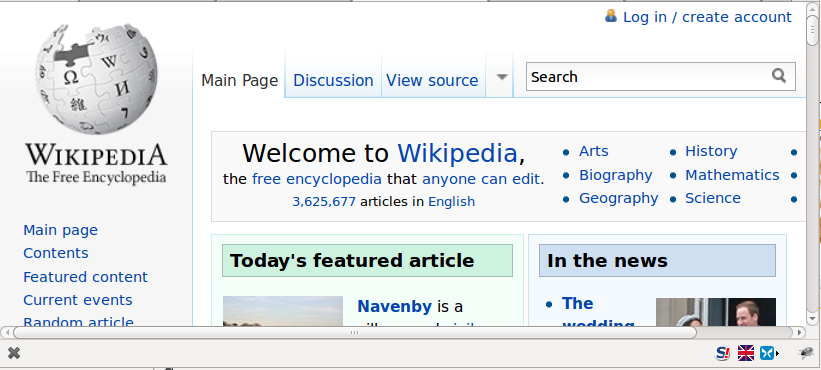
\includegraphics[scale=0.4]{../task05/wikipedia_homepage.png} 
  \caption{The language of en.wikipedia.org is correctly recognized as english}
  \label{f:wpHomepage}
\end{center}
\end{figure}
	
\end{frame}

\begin{frame}[c]
	\myframetitle{Firefox Plugin for language detection}{Norwegian}
	%\usepackage{graphics} is needed for \includegraphics
\begin{figure}[htp]
\begin{center}
  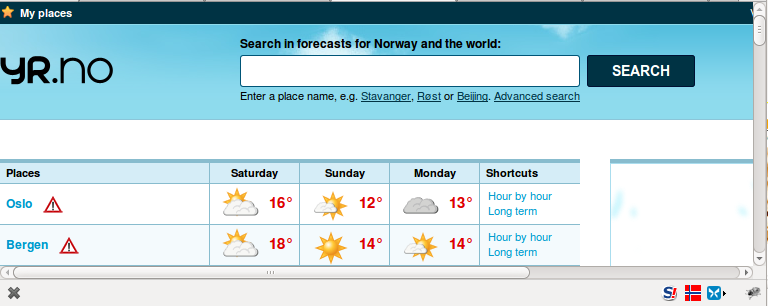
\includegraphics[scale=0.4]{../task05/yr_homepage.png} 
  \caption{The plugin detects norwegian as the language of the weather
  site yr.no}
  \label{figureLabel}
\end{center}
\end{figure}
	
\end{frame}

\begin{frame}[c]
	\myframetitle{Firefox Plugin for language detection}{Failure if p-Tag is
	missing}
	%\usepackage{graphics} is needed for \includegraphics
\begin{figure}[htp]
\begin{center}
  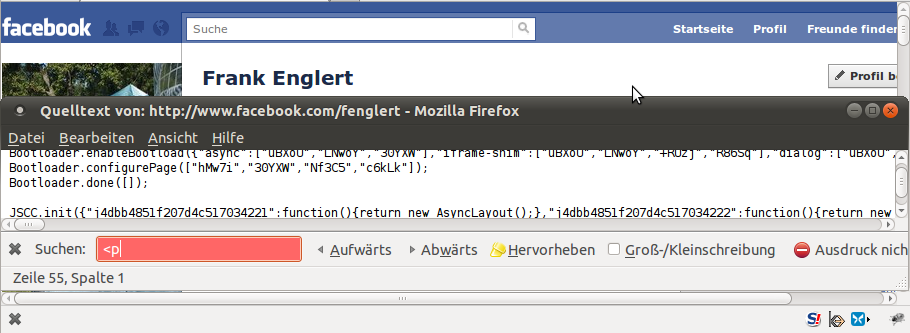
\includegraphics[scale=0.35]{../task05/facebook_homepage.png} 
  \caption{The detection fails if there are no p-Tags indicated by the KE logo}
  \label{figureLabel}
\end{center}
\end{figure}
	
\end{frame}



\begin{frame}[c]
	\myframetitle{Firefox Plugin for language detection}{How it works}
	
	\begin{itemize}
	\fatitem{Implementation details}
	
	\begin{itemize}
		\item Split the text between the '<p>' and '</p>' tags
		\item Count the occurrence of the stop words for german, english and norwegian
		\item Display the icon for the language with the most stop words
	\end{itemize}
		\item ca. 15 LoC without stop word dictionaries
		\fatitem{ good results for such a simple heuristic }
\end{itemize}
\end{frame}

\begin{frame}[c]
\myframetitle{Firefox Plugin for language detection}{Surf session results}
	\begin{table}
		\begin{tabular}{|l|l|l|l|l|}
		\hline 
		URL & \multicolumn{3}{|c|}{Number of stop words} & Correct? \\
		\hline 
		 & de & en & no & \\
		 \hline 
		heise.de & 308 & 18 & 29 & yes\\
		faz.de & 232 & 20 & 21 & yes\\
		ke.tud/.../webmining & 106 & 10 & 14 & yes\\
		gnome.org & 1 & 23 & 1 & yes\\
		kernel.org & 18 & 635 & 37 & yes\\
		yr.no & 10 & 43 & 36 & yes\\
		dagbladet.no & 105 & 548 & 921 & yes\\
		facebook.com/fenglert & 0 & 0 & 0 & no\\
		se.wikipedia.org & 2 & 1 & 0 & -- \\
		fr.wikipedia.org & 22 & 44 & 2 & -- \\
		ja.wikipedia.org & 0 & 0 & 0 & -- \\
		\hline 
		\end{tabular}
		\caption{Language detection Results for a short surf session}
		\label{tblFFPluginResults}
	\end{table}
\end{frame}

\begin{frame}[c]
	\myframetitle{Firefox Plugin for language detection}{Test results}
	\begin{itemize}
	  \fatitem{The results are quite good!}
      \fatitem{ Language correctly detected}
      \begin{itemize}
      	\item on 7 of 8 pages
	  \end{itemize}
      
      \fatitem{But:}
      \begin{itemize}
      	\item Some pages contains multiple languages. e.g yr.no
      	\item The detection fails if a page contains no p-Tags
      	\item The detection yields bogus results if there are no rules for a
      language
	  \end{itemize}
    \end{itemize}
\end{frame}
